%!TEX TS-program = xelatex  
%!TEX encoding = UTF-8 Unicode  
\documentclass[12pt,a4paper]{paper}
\usepackage{float}
\usepackage{indentfirst}
\usepackage{geometry} 
\usepackage{enumitem} 
\usepackage{amsmath}  
\usepackage{braket}    
\usepackage{fontspec,xltxtra,xunicode} 


\usepackage[]{xeCJK}
\setCJKmainfont[ItalicFont=STHeitiSC-Light]{STSong}
\setCJKsansfont[BoldFont=STHeiti]{STXihei}
\setCJKmonofont{STFangsong}

%\defaultfontfeatures{Mapping=tex-text}  
%\setromanfont{SimSun} %设置中文字体  
\XeTeXlinebreaklocale “zh”  
\XeTeXlinebreakskip = 0pt plus 1pt minus 0.1pt %文章内中文自动换行  
      

\title{Black-Scholes Formula, a physicist's perspective}
\author{}
\date{\today}
\begin{document}
\maketitle
\section{(a)}
Rewritten Using $Brownian$ $Motion$: 
\begin{equation}
ds(t) = \phi s(t) dt + \sigma s(t) dW(t).
\end{equation}
where $W(t)$ is a standard brownian motion.\\\indent To illustrate the relation between \textbf{Gaussian Noise} and \textbf{Brownian Motion}, consider when using $R(t)$, we're actually suggesting $s(t + \epsilon) = s(t) + \phi s(t) \epsilon + \sigma R \epsilon$. In this case, $R \sim \mathcal{N}(0, \frac{1}{\epsilon})$, therefore $R \epsilon \sim \mathcal{N}(0, \epsilon)$, which can be characterized as $W(t + \epsilon) - W(t)$. As $\epsilon \rightarrow 0$, $W(t + \epsilon) - W(t) \rightarrow dW(t)$. (It's really clearer to use $brownian$ $motion$ notation.) Brownian motion has the property that $dW(t)dW(t) = dt$, $dW(t) dt = 0$.\\
\indent The original statement can be rewritten as: 
\begin{equation}
df(t, s(t)) = f_t dt + \frac{1}{2}\sigma^2s^2f_{ss}dt + \phi s f_s dt + \sigma s dW(t).
\end{equation}
\indent According to $Taylor$ $expansion$ $formula$, we can write
\begin{equation} 
df = f_t dt + f_s ds + \frac{1}{2}\{f_{tt} dt^2 + (f_{ts} + f_{st})dt ds(t) + f_{ss} ds(t)ds(t) \} + o(dt^2)
\end{equation} 

\begin{equation}
\Longrightarrow df = f_t dt + f_s ds + \frac{1}{2} f_{ss} ds(t)ds(t)
\end{equation}

\indent Considering $ds(t) = \phi s(t) dt + \sigma s(t) dW(t)$, $dW(t)dW(t) = dt$, $dW(t) dt = 0$, we have 
\begin{equation}
df = f_t dt + \frac{1}{2}\sigma^2s^2f_{ss}dt + \phi s f_s dt + \sigma s dW(t)
\end{equation}
\indent Using the relationship between W(t) and R(t), we can change dW(t) and derive:
\begin{equation}
\frac{df}{dt}=\frac{\partial f}{\partial t}+\frac{1}{2}\sigma ^{2}s^{2}\frac{\partial^2 f}{\partial s^2}+\frac{\partial f}{\partial s}(\phi s+\sigma sR).
\end{equation}

\section{(b)}
\indent We've already known that $c = c(t, s(t))$. Consider a portfolio $\Pi=c-\frac{\partial c}{\partial s}s$.\\
\indent To calculate the derivative of $\Pi$ we can write down the differential of $\Pi$:
\begin{equation}
d\Pi = c_t dt + c_s ds + \frac{1}{2}c_{ss} ds ds - c_s ds.
\end{equation}
\indent Because we've got $dS^2={\sigma}^{2} s^{2}dt$, we can derive:
\begin{equation}
\frac{d\Pi}{dt}= c_t + \frac{1}{2} c_{ss} \sigma^2 s^2.
\end{equation}

\section{(c)}
\indent r means the short-term risk-free interest rate. The following equation must be true:
\begin{equation}
\frac{d\Pi}{dt}=r\Pi.
\end{equation}
\indent Otherwise arbitrage will exist, which contradicts our assumption. Therefore we can write $d\Pi = r(c - c_s s)dt$. It's equivalent to the previous result $c_t dt + \frac{1}{2} c_{ss} \sigma^2 s^2 dt$.\\
\indent At last we have the \textbf{Black-Scholes formula}:
\begin{equation}
c_t + \frac{1}{2}\sigma^2 s^2 c_{ss} + rsc_s - rc = 0.
\end{equation}
\indent Why the equation does not contain \phi?


\section*{Another Way of Obtaining B-S Formula}
According to non-arbitrage postulate, if at time $0$, $c(0, S(0)) = c_0$, then we should should be able to construct a portfolio $X(t)$(with $X(0) = c_0$) to replicate exactly this option. We should use the underlying stock $S(t)$ and the money market with interest rate $r$. Suppose we hold $\Delta(t)$ share of stock at time $t$, then it follows:
\begin{equation}
dX(t) = \Delta(t)dS(t) + r(X(t) - \Delta(t)S(t))dt = D_tdt + D_w dW(t)
\end{equation}
where $D_t = \Delta(t)S(t)(\phi - r) + r X(t)$, $D_w = \Delta(t)S(t)\sigma$.\\
\indent At the same time,
\begin{equation}
dc(t, S(t)) = c_t dt + c_s dS(t) + \frac{1}{2} c_{ss} dS(t)dS(t) = D_t' dt + D_w'dW(t)
\end{equation}
where $D_t' = c_t + c_s \phi S(t) + \frac{1}{2}\sigma^2 S(t)^2c_{ss}$, $D_w' = c_s \sigma S(t)$. \\
\indent Therefore, it should follows that $D_t = D_t', D_w = D_w'$. The second relation yields instantly that $\Delta(t) = c_s$, while the first would amount to the Black-Scholes formula:
\begin{equation}
c_t + \frac{1}{2}\sigma^2 s^2 c_{ss} + rsc_s - rc = 0
\end{equation}

\section{(d)}
Change variable $s = e^x$, we have:
\begin{equation}
c_x = e^{-x}c_s.
\end{equation}
\begin{equation}
c_t = rc - rsc_s - \frac{1}{2}\sigma^2 s^2 c_{ss} = (r - (r - \frac{1}{2}\sigma^2)\frac{\partial}{\partial x} - \frac{1}{2}\sigma^2 \frac{\partial^2}{\partial x^2}) c.
\end{equation}
\indent Therefore we can easily prove that
\begin{equation} 
H_{BS} = (1 - \frac{\partial}{\partial x})(r + \frac{1}{2} \sigma^2 \frac{\partial}{\partial x})=-\frac{\sigma ^2}{2}\frac{\partial^2 }{\partial x^2}+(\frac{\sigma ^2}{2}-r)\frac{\partial }{\partial x}+r. 
\end{equation}
which is the Hamiltonian for Black-Scholes model.

\section{(e)}
\begin{equation}
p_{BS}(x, \tau; x') = \braket{x|e^{-\tau H}|x'} = \int_{\infty}^{\infty} \frac{dp}{2\pi}\braket{x|e^{-\tau H}|p}\braket{p|x'}
\end{equation}
Taking $p = i \frac{\partial}{\partial x}$, using $\braket{x|p} = e^{ipx}$:
\begin{equation}
p_{BS}(x, \tau;x') = e^{-r\tau}\int_{\infty}^{\infty}\frac{dp}{2\pi}exp\{- \frac{1}{2}\sigma^2p^2\tau + ip(x - x') + ip\tau(r - \frac{\sigma^2}{2}) \}
\end{equation}
Finally, perform the Gaussian integration:
\begin{equation}
p_{BS}(x, \tau;x') = e^{-r\tau} \frac{1}{\sqrt{2\pi \tau \sigma^2}} exp\{ - \frac{1}{2 \sigma^2 \tau}(x - x' + \tau(r - \frac{\sigma^2}{2}) )^2 \}
\end{equation}

\section{(f)}
After obtaining the pricing kernel, we can get the price of call option at time $t$ simply by integrating the final value with the kernel.
\begin{equation}
c(\tau, x) = \int_{- \infty}^{\infty} g(x') P_{BS} dx'
\end{equation}
where in this case, $g(x') = (e^{x'} - K)^{+}$. $(x)^{+}$ takes $x$ when $x > 0$ and takes $0$ when $x \leq 0$. Therefore, the integration only takes place in $x \in (lnK, \infty)$.\par
After noticing, the pricing kernel is actually $e^{-r \tau}$ mutilpying a normal distribution, we can define $d_{-}(\tau, x) = \frac{1}{\sigma\sqrt{\tau}} [\frac{x}{lnK} + (r - \frac{1}{2}\sigma^2)\tau], d_{+} = d_{-} + \sigma \sqrt{\tau}$, $N(x) = \frac{1}{\sqrt{2\pi}}\int_{-\infty}^x e^{-\frac{x^2}{2}}$. We separate the integration into two parts: $K$ and $e^x$.\par
\begin{subequations}
\begin{align}
\int_{lnK}^{\infty} K P_{BS} dx' &= e^{-r\tau}KN(d_{-}(\tau, x)) \\
\int_{lnK}^{\infty} e^x P_{BS} dx' &= e^{x}N(d_{+}(\tau, x))
\end{align}
\end{subequations}
Remember that $s = e^{x}$, we have the pricing formula for $c(t, s)$:
\begin{equation}
c(t, s) = sN(d_{+}(\tau, s)) - e^{-r\tau} K N(d_{-}(\tau, s))
\end{equation}

With this formula, we can plot the time-evolution of stock prices and call option prices.\par
The following code does the job in $R$, results shown in $fig.1 \sim 3$
\begin{verbatim}
c_time_evolution <- function(sigma, x0, r, K)
{
    tau = seq(0, 1, 0.01)[-1]
    w = rnorm(100, 0, 0.01)
    w = cumsum(w)
    # calculate s(t)
    x = (r - 0.5*sigma^2) * tau + sigma * w
    x = exp(x)
    x = x0 * x
    #fi
    plot(tau, x, type='l')
    
    d1 = log(x/K) + (1 - tau) * (r + 0.5*sigma^2)
    d1 = d1/(sqrt(1 - tau) * sigma)
    d2 = d1 - sigma*sqrt(1 - tau)
    c = x * pnorm(d1) - exp(-r * (1-tau)) * K * pnorm(d2)
    plot(tau, c, 'l')
}
#fig.1
c_time_evolution(sigma = 0.5, x0 = 100, r = 0.20, K = 100)
#fig.2
c_time_evolution(sigma = 0.5, x0 = 80, r = 0.20, K = 100)
#fig.3
c_time_evolution(sigma = 0.5, x0 = 120, r = 0.20, K = 100)
\end{verbatim}

\begin{figure}[H]
\caption{Time-evolution of call option price}
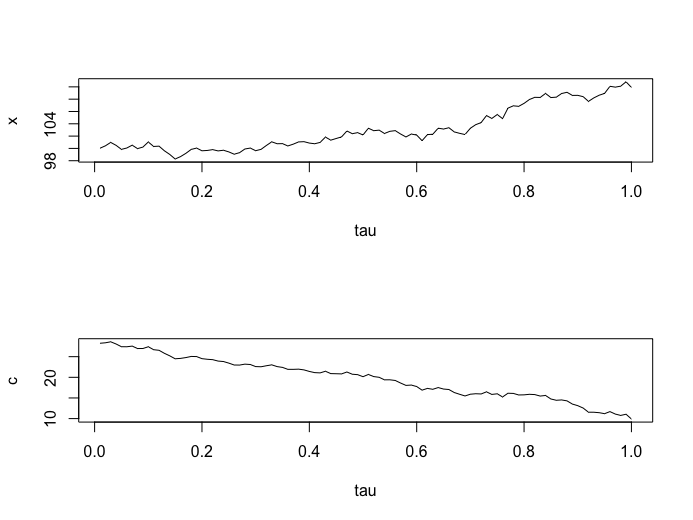
\includegraphics[scale = 0.6]{figure1.png}
\end{figure}


\begin{figure}[H]
\caption{Time-evolution of call option price}
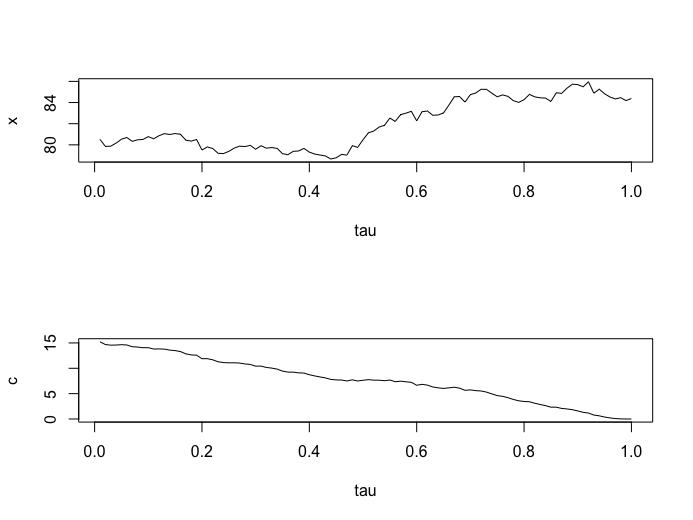
\includegraphics[scale = 0.6]{figure2.png}
\end{figure}


\begin{figure}[H]
\caption{Time-evolution of call option price}
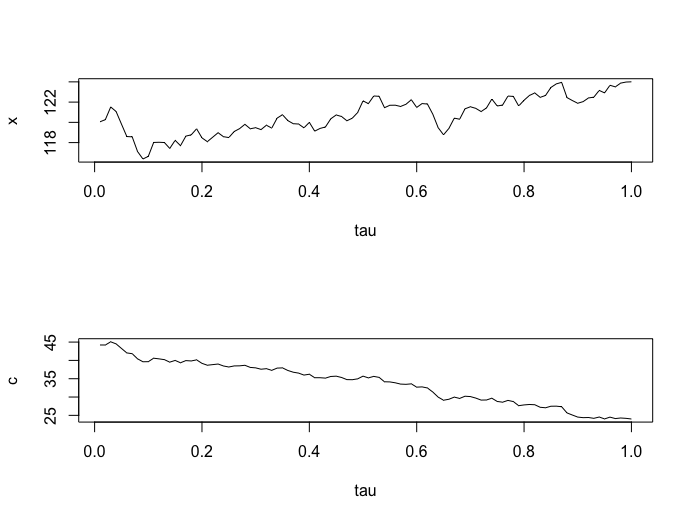
\includegraphics[scale = 0.6]{figure3.png}
\end{figure}

As shown in these figures, call option price drops as $(T-t)$ decreases.

\section{(g)}
\indent Consider a down-and-out barrier European option. If $s\leq e^B(x\leq B)$ it will become worthless, which means $c=0$. \\
\indent For an arbitrary potential $v(x)$, we have:$\frac{\partial c}{\partial t}=Hc$, where $H$ can be written as:
\begin{equation}
H=-\frac{\sigma ^2}{2}\frac{\partial^2 }{\partial x^2}+(\frac{\sigma^2}{2} -r)\frac{\partial }{\partial x}+V(x).
\end{equation}
\indent Obviously, if we set $V(x)=\infty$ when $x\leq B$, then $c=0$ is automaticlly satisfied. However, when $x>B$, the changing of $c$ still conform to the B-S formula. comparing with $H_{BS}$, we have:
V(x)=
$\left\{\begin{matrix}
+\infty,x\leq B.\\
r,x>B.
\end{matrix}\right.$

\section{(h)}
\indent The Hamiltonian for the down and out option is given by:
\begin{equation}
H_{DO}=H_{BS}+V(x)=\frac{\sigma ^2}{2}\frac{\partial ^2}{\partial x^2}+(\frac{\sigma ^2}{2}-r)\frac{\partial}{\partial x}+V(x)
\end{equation}
V(x) is defined in $(g)$.\\
\indent Now we can construct the eigenfunctions similar to the $Black-Scholes$ case except that these must satisfy $\Psi _{E}(B)=0$.\\
\indent Define the quantities:
\begin{equation}
\beta =\frac{(\frac{\sigma ^2 }{2}+r)^2}{\sigma ^4}, p=\sqrt{\frac{2E}{\sigma ^2}-\beta},\alpha =\frac{\frac{\sigma ^2}{2}-r}{\sigma ^2}, i\lambda _{\pm}=\alpha \pm ip
\end{equation}
\indent The eigenfunctions are given by:
\begin{equation}
x>B:\langle x|\Psi_{E}\rangle =e^{i\lambda_{+}(x-B)}-e^{i\lambda_{-}(x-B)}=2ie^{\alpha (x-B)}\sin{[p(x-B)]}
\end{equation}
\begin{equation}
\langle \widetilde{\Psi_{E}}|x\rangle =e^{-i\lambda_{+}(x-B)}-e^{-i\lambda_{-}(x-B)}=-2ie^{-\alpha (x-B)}\sin{[p(x-B)]}
\end{equation}
\begin{equation}
\left \langle \widetilde{\Psi _{E}} | {\Psi_{E}}' \right \rangle=[2\pi \sigma ^2 \sqrt{2E/\sigma ^2 -\beta }] \delta (E-{E}').
\end{equation}
\begin{equation}
x \leq B: \left \langle x | \Psi _{E} \right \rangle=0=\left \langle \widetilde{\Psi _{E}} | x \right \rangle.
\end{equation}
\indent Now we can use the eigenfunctions to evaluate the pricing kernel. Again we work with the p variable:
\begin{align*}
\ p_{DO}(x,\tau;{x}')\
& =  \left \langle x | e^{-\tau H_{DO}} | {x}' \right \rangle \\
& = e^{-\frac{\tau \beta \sigma ^2}{2}+\alpha (x-{x}')}\int_{0}^{\infty }\frac{dp}{2\pi }e^{-\frac{1}{2}\tau \sigma ^2 p^2} [e^{ip(x-{x}')}+e^{-ip(x-{x}')}\\
& -e^{ip(x+{x}'-2B)}-e^{-ip(x+{x}'-2B)}].\
\end{align*}
\indent Consider that we have already derived:
\begin{equation}
p_{BS}(x,\tau;{x}')=e^{-r\tau}\frac{1}{\sqrt{2\pi \tau \sigma ^2}}e^{-\frac{1}{2\tau \sigma ^2}[x-{x}'+\tau(r-\frac{\sigma ^2}{2})]^2}.
\end{equation}
We can simplify the pricing kernel using the previous results:
\begin{equation}
p_{DO}(x,\tau;{x}')=p_{BS}(x,\tau;{x}')-(\frac{e^{x}}{e^{B}})^{2\alpha } p_{BS}(2B-x,\tau;{x}').
\end{equation}

\section{(i)}
We know that $r(t)$ satisfied Langevin equation:
\begin{equation}
\frac{dr}{dt}=a(r,t)+\sigma (r,t)R(t).
\end{equation}
\indent Here $R(t)$ is still Gaussian noise.\\
\indent Define the propagator $P(r,t;r_{0})$: if $r(t_0)=r_0$, the probability of $r(t)=r$ equals $P(r,t;r_{0})$.\\
\indent From the Langevin equation we have:
\begin {equation}
r(t+\varepsilon )=r(t)+\varepsilon [a+\sigma R(t)].
\end{equation}
Change it into the following formula:
\begin {equation}
r={r}'+\varepsilon [a({r}')+\sigma ({r}')R(t)].
\end{equation}
\indent Thus we can calculate the propagator:
\begin {align*}
\ P(r,t+\varepsilon ,r_{0})
& =P({r}',t;r_{0})|_{{r}'=r-\varepsilon [a({r}')+\sigma ({r}')R(t)]}\\
 &=\int P({r}',t;r_{0})\delta (r-{r}'-\varepsilon [a({r}')+\sigma ({r}')R(t)])d{r}'\\
 & \simeq \int P({r}',t;r_{0})d{r}'\{\delta (r-{r}') +\frac{\partial \delta (r-{r}')}{\partial {r}'}\varepsilon [a({r}')+\sigma ({r}')R(t)] \\
&+ \frac{1}{2}\frac{\partial^2 \delta (r-{r}')}{\partial {r}'^2} \varepsilon ^2 [a({r}')+\sigma ({r}')R(t)]^2 +... \}.\
\end{align*}
\indent Because $<R^2(t)>=\frac{1}{\varepsilon}$ and $<R(t)>=0$, the previous formula can be re-written like this:
\begin{align*}
\ P(r,t+\varepsilon ,r_{0})
& =P({r}',t;r_{0})+\int d{r}'P({r}',t;r_{0}) \{ \frac{\partial \delta (r-{r}')}{\partial {r}'}\varepsilon a({r}')+\frac{1}{2}\frac{\partial^2 \delta (r-{r}')}{\partial {r}'^2}\varepsilon ^2 \sigma ^2({r}')\frac{1}{\varepsilon } \} \\
& = P({r}',t;r_{0})-\varepsilon \frac{\partial }{\partial r}[a(r)P(r,t;r_0)]+\frac{\varepsilon }{2}\frac{\partial^2 }{\partial r^2}[\sigma (r)^2 P(r,t;r_0)].\
\end{align*}
\indent If a variable is o($\varepsilon$), it is automatically neglected.\\
\indent Thus, from the definition of derivative, we have:
\begin{equation}
\frac{\partial P(r,t;r_0)}{\partial t}=[\frac{1}{2}\frac{\partial^2 }{\partial r^2}\sigma ^2(r)-\frac{\partial }{\partial r}a(r)]P(r,t;r_0).
\end {equation}
\indent We've already known that:
\begin{equation}
\frac{\partial P(r,t;r_0)}{\partial t}=-H_{F}P(r,t;r_0).
\end{equation}
Therefore we can prove:
\begin{equation}
H_{F}=-\frac{1}{2}\frac{\partial^2 }{\partial r^2}\sigma ^2(r)+\frac{\partial }{\partial r}a(r)=-\frac{1}{2}\frac{\partial^2 }{\partial r^2}\sigma ^2(r)+a(r)\frac{\partial }{\partial r}+\frac{\partial a(r)}{\partial r}.
\end{equation}
\indent From a different perspective, we define $P_{B}(R,t;r)$ as the back propagator.\\
\indent Similarly we have( since the time flows backwards this time):
\begin{equation}
\frac{\partial P_{B}(R,t;r)}{\partial t}=+H_{B}P_{B}(R,t;r).
\end{equation}
\indent Finally we can calculate:
\begin{equation}
H_{B}=-\frac{1}{2}\sigma ^2(r)\frac{\partial^2 }{\partial r^2}-a(r)\frac{\partial }{\partial r}.
\end{equation}
$H_{B}=H_{F}^{\dag}$ is obvious.

\section{(j)}
In this part we'll focus on the so-called \textbf{stochastic Quantization}.\\
\indent The Langevin equation:
\begin{equation}
\frac{dr}{dt}=a(r,t)+\sigma (r.t)R(t)
\end{equation}
is satisfied at any time between $t_{0}$ and $T$. We must consider that both $r$ and $R$ are stochastic variables. Therefore when calculating $z_{B}$( can be compared to partition function in statistical mechanics), we must integrate over all possible paths
\begin{equation}
Z_{B}=\int DRDr\prod_{t=t_{0}}^T \delta [\frac{dr}{dc}-a(r,t)-\sigma (r,t)R(t)]e^-\frac{1}{2}\int_{t_{0}}^{T}R^2 (t)dt
\end{equation}
$Dr$ means integrating over all possible $r(t): \int Dr=\int_{-\infty}^{+\infty} \prod_{t=t_{0}}^T dr(t)$.\\
\indent We hope to write $Z_{B}$ int the form of $z_{B}=\int Dre^{s_{B}}$. Because of this, we calculate the integral over $R$ first:
\begin{equation}
Z_{B}=\int Drexp(-\frac{1}{2}\int_{t_{0}}^T \frac{[\frac{dr}{dt}-a(r,t)]^2}{\sigma^2 (r,t)}dt).
\end{equation}
\indent Because the $Dirac-\delta$ function makes sure we only keep $R(t)$ that satisfies the Langevin equation: $R(t)=\frac{\frac{dr}{dt}-a(r,t)}{\sigma (r,t)}$.\\
\indent It's easy to calculate $S_{B}$:
\begin{equation}
S_{B}=-\frac{1}{2}\int_{t_{0}}^T \frac{[\frac{dr}{dt}-a(r,t)]^2}{\sigma^2 (r,t)}dt.
\end{equation}
\indent From the definition of $S_{B}:S_{B}=\int_{t_{0}}^T Ldt,$ it's clear that:
\begin{equation}
L=-\frac{[\frac{dr}{dt}-a(r,t)]^2}{2\sigma^2 (r,t)}dt.
\end{equation}

\section{(k)}
The Vasicek model can be described using the following equation:
\begin{equation}
\frac{dr}{dt}=a(b-r)+\sigma R(t).
\end{equation}
\indent Note that if we set 
$\left\{\begin{matrix}
a(r,t)=a(b-r).\\
\sigma (r,t)=\sigma .
\end{matrix}\right.$ in Langevin equation( $a$,$b$,$\sigma$ are all constants), we have the Vasicek model naturally.\\
\indent Thus we get:
\begin{equation}
L_{V}=-\frac{[\frac{dr}{dt}-a(b-r)]^2}{2\sigma ^2}.
\end{equation}
\begin{equation}
S_{V}=-\frac{1}{2\sigma ^2}\int_{t_0}^{T}[\frac{dr}{dt}-a(b-r)]^2 dt.
\end{equation}
In the next section we'll use $S_{V}$ to calculate the propagator of Vasicek model.

\section{(l)}
\indent For different paths(which all have different $S_{V}$), so that ${e^{S_{V}}/Z}$ is the distribution of probability. $Z=\int Dr e^{S_{V}}.$
\indent Given by the question itself, we know that the propagator equals:
\begin{equation}
P(t_{0},T)=\frac{1}{Z}\int Dr e^{S_{V}} e^{-\int_{t_{0}}^{T} r(t)dt}.
\end{equation}
\indent If we use a new variable $S=S_{V}-\int_{t_{0}}^{T} r(t)dt$, then we have:
\begin{equation}
P(t_{0},T)=\frac{1}{Z}\int Dr e^{S}.
\end{equation}
\indent Change the variable: $u=r-b$. Thus we can write:
\begin{align*}
S=&-\frac{1}{2\sigma ^2}\int_{t_{0}}^{T}dt[\frac{du}{dt}+au]^2 -\int_{t_{0}}^{T}(u+b)dt\\
& =-\frac{1}{2\sigma ^2}\int_{t_{0}}^{T}dt[\frac{dr}{dt}+ar]^2 -\int_{t_{0}}^{T}(r+b)dt.
\end{align*}
\indent Next, we can define $v(t)=ar(t)+\frac{dr(t)}{dt}$. View this formula as a differential equation of $r(t)$:
\begin{equation}
\frac{dr}{dt}+ar=v(t).
\end{equation}
The solution can be easily derived:
\begin{equation}
r(t)=e^{-a(t-t_{0})}r_{0}+e^{-at}\int_{t_{0}}^{t}e^{a{t}'}v({t}')d{t}'.
\end{equation}
\indent Since we want to calculate the integral of r(t), we now have:
\begin{equation}
\int_{t_{0}}^{T}r(t)dt=B(t_{0},T)r_{0} + \int_{t_{0}}^{T} B(t,T)v(t)dt.
\end{equation}
where $B(t,T)=\frac{1-e^{-a(T-t)}}{a}$.\\
\indent From the definition of $v(t)$ we can tell that $v(T)$ is free to take all possible values. Therefore we can use the following path integral to calculate propagator:
\begin{align*}
P(t_{0}, T) &=e^{-b(T-t_{0})-B(t_{0},T)r_{0}} \frac{1}{Z}\int Dv e^{-\frac{1}{2\sigma ^2}\int_{t_0}^{T}dt[v(t)^2 + 2\sigma ^2 B(t,T)v(t)]}\\
& =e^{-b(T-t_{0})-B(t_{0},T)r_{0}} e^{\frac{\sigma ^2}{2}\int_{t_{0}}^{T}dt B(t,T)^2}.
\end{align*}
\indent The $v(t)$ integrations are decoupled Gaussian integrations, with the overall normalization being canceled by the factor Z.\\
\indent Finally, assume $B(\theta)=\frac{1-e^{-a\theta}}{a}$, where $\theta=T-t_{0}$, and $A(\theta)=exp[(\frac{\sigma^2}{2a^2}-b)(\theta -B(\theta))-\frac{\sigma ^2}{4a}B(\theta)^2]$.\\
\begin{equation}
A(\theta)e^{-r_{0}B(\theta)}=exp[-b\theta-r_{0}\frac{1-e^{-a\theta}}{a}+\frac{\sigma ^2}{2a^2}\theta - \frac{\sigma ^2 (1-e^{-a\theta})}{2a^3} +\frac{b}{a}(1-e^{-a\theta})-\frac{\sigma ^2}{4a^3}(1-e^{-a\theta})^2].
\end{equation}
\indent If we want to prove $P(t_{0},T)=A(\theta)e^{-r_{0}B(\theta)}$, then we must prove:

\begin{align*}
-b(T-t_{0})-B(t_{0},T)r_{0} +\frac{\sigma ^2}{2}& \int_{t_{0}}^{T}dt B(t,T)^2 =-b\theta-r_{0}\frac{1-e^{-a\theta}}{a}+\frac{\sigma ^2}{2a^2}\theta \\
& - \frac{\sigma ^2 (1-e^{-a\theta})}{2a^3} +\frac{b}{a}(1-e^{-a\theta})-\frac{\sigma ^2}{4a^3}(1-e^{-a\theta})^2.
\end{align*}

Change all $T-t_{0}$ to $\theta$ and all $B(t_{0},T)$ to $B(\theta)$, and calculate the integral of $B(\theta)$, we can simplify the equation:
\begin{equation}
\int_{t_{0}}^{T}\frac{(1-e^{-a\theta})^2}{a^2}dt=\frac{\theta}{a^2}-\frac{1-e^{-a\theta}}{a^3}+\frac{2b}{a\sigma ^2}(1-e^{-a\theta})-\frac{(1-e^{-a\theta})^2}{2a^3}.
\end{equation}
the left side can be written as:
\begin{equation}
\int_{t_{0}}^{T}\frac{(1-e^{-a\theta})^2}{a^2}dt=\frac{\theta}{a^2}-\frac{2}{a^3}e^{-aT}(e^{aT}-e^{at_{0}})+\frac{1}{2a^3}e^{-2aT}(e^{2aT}-e^{2at_{0}}).
\end {equation}
\indent After some comparison, the correctness is easy to prove.

\section{Conclusion}

\section{Reference}
[1]Belal E.Baaquie, Quantum Finance: Path integrals and Hamiltonians for Options and Interest Rates. Cambridge University Press (2004).
[2]Zee.A, Quantum field theory in a nutshell. Princeton university press (2010).
[3]J. C. Hull, Options, Futures and Other Derivatives. Fifth Edition, Prentice-Hall International (2003).
[4]M. Otto, ‘Using path integrals to price interest rate derivatives’, http://xxx.lanl.gov/cond-mat/9812318.
[5]O. Vasicek, ‘An Equilibrium Characterization of the Term Structure’. Journal of Financial Economics, 5: 177.
\end{document}
